\newcommand{\dST}{\Delta\fdot_{T}}
\renewcommand{\tref}{t_{\textrm{R}}}

\newcommand{\two}[2]{
\left\{
\begin{array}{cc}
#1  &t \in A \\
#2& t \in B
\end{array}•
\right.}

%\subsection{Calculating the mismatch}
%\textcolor{red}{Here is a derivation - better to use the mismatch framework worked out in the last chapter.}
%Having obtained the phase residual we know proceed to calculate the mismatch which would be
%induced for a CW search. 
%Initially lets consider the mismatch over a single cycle such that the observation time is $T_{\textrm{obs}} =T$.
%Then the matched filtering amplitude can be calculated by subdomaining the intergral into contribution
%when in the $A$ domain and those in $B$
%\begin{align}
%X & = \frac{1}{T}\left(\int_{A}e^{i\Delta\Phi(t)} dt + \int_{B}e^{i\Delta\Phi(t)} dt\right)
%\label{eqn: matched filtering amplitude}
%\end{align}•
%The form of the phase residual in equation~\eqref{eqn: full phase residual} does not allow for an easy integration.
%We can proceed by considering the limit  $\Delta\f_{T} \rightarrow 0$ and Taylor expand equation~\eqref{eqn: full phase residual} about this point
%\begin{align}
%\int_{A}e^{i\Delta\Phi(t)} dt & \approx \int_{0}^{RT} 1 + i\pi(1-R)t\left(t-RT\right)\dST +
%\frac{i^{2}\pi^{2}}{2}\left(1-R\right)^{2}t^{2}(t-RT)^{2}\dST^{2} dt \ntag\\
%&\approx RT - i\frac{\pi}{6} \dST R^{3}T^{3}(1-R) - \frac{\pi^{2}}{60}\dST^{2}(1-R)^{2}R^{5}T^{5}\\
%\int_{B}e^{i\Delta\Phi(t)} dt & \approx \int_{RT}^{T} 1 - i\pi R\left((t-T)(t-RT)\right) \dST+ \frac{i^{2}\pi^{2}}{2}R^{2}(t-T)^{2}(t-RT)^{2}\dST^{2} dt\\
%&\approx T(1-R) +  i\frac{\pi}{6} \dST T^{3}R(1-R)^{3} - \frac{\pi^{2}}{60}\dST^{2}T^{5}R^{2}(1-R)^{5}.
%\end{align}
%The matched filtering amplitude 
%over one cycle is then
%\begin{align}
%X &\approx 1 + i\frac{\pi}{6} \dST T^{2}\left(R(1-R)^{3} - R^{3}(1-R)\right) - \frac{\pi^{2}}{60}\dST^{2}T^{4}\left((1-R)^{2}R^{5} + R^{2}(1-R)^{5}\right) + \mathcal{O}\left(\Delta{\dot\f_{A}}^{2}\right). \\
%& \approx 1 + i\frac{\pi}{6} \dST T^{2}R\left(1-2R\right)\left(1-R\right) - \frac{\pi^{2}}{60}\dST^{2}T^{4}R^{2}(R-1)^{2}(3R^{2}-3R+1)+ \mathcal{O}\left(\Delta{\dot\f_{A}}^{2}\right).
%\end{align}
%The mismatch is then given by
%\begin{align}
%m & =1 - |X|^{2} \\
% & \approx  1 - \left|
%\left(1 - \frac{\pi^{2}}{60}\dST^{2}T^{4}R^{2}(1-R)^{2}(3R^{2} - 3R +1) \right)^{2} + \left(\frac{\pi}{6} \dST T^{2} R\left(1-2R\right)\left(1-R\right) \right)^{2}\right| \\
%& \approx \pi^{2}\dST^{2}T^{4}(1-R)^{2}R^{2}\left| \frac{1}{36}\left(1-2R\right)^{2} - \frac{1}{30}\left(3R^{2}-3R+1\right)\right| \\
%& \approx \frac{\pi^{2}}{180}\dST^{2}T^{4}(1-R)^{2}R^{2}\left|2R^{2} - 2R -1\right| 
%+ \mathcal{O}(\dST^{3})
%\label{eqn: Lyne mismatch}
%\end{align}

\subsection{Calculating the mismatch}
Writing the parameter space offsets in terms of the total spin-down variation
\begin{align}
\Delta\fdot(t) &= \dST\two{1-R}{-R} \\
\Delta\f(t) &= 0  \\
\Delta\phi(t) & = \frac{\pi}{4} \dST T^{2}(1-R)R \two{-R}{1-R},
\label{eqn: Lyne parameter space offsets}
\end{align}
note that the parameter space offsets vary discreetly with time. Combining
these into the quantity 
\begin{equation}
\bdl^{\alpha i} = \left[\bdl_{A}, \bdl_{B}\right].
\end{equation}
Then the mismatch over a single cycle can be calculated from
\begin{align}
m = & g_{\alpha\beta ij}\bdl^{\alpha i} \bdl^{\beta j},
\end{align}
where $g_{\alpha\beta i j}$ can be calculated from equation~\eqref{eqn: metric}
using the reference times for each subdomain and setting the observation time
from $t=0$ to $t=T$ (e.g. one cycle). Substituting the correct expression in we find a mismatch given by
\begin{equation}
m = \frac{\pi^{2} R^{2}}{180} T^{4} \dST^{2} \left(R - 1\right)^{2} 
    \left(-2 R^{2} + 2 R + 1\right)
\label{eqn: mismatch lyne single switch}
\end{equation}•

This is illustrated in Fig.~\ref{fig: Lyne mismatch} for the valid range of R
demonstrating that the mismatch is maximal when the two periods are equal and
vanishes when either duration tends to zero as expected.

\begin{figure}[ht]
\centering
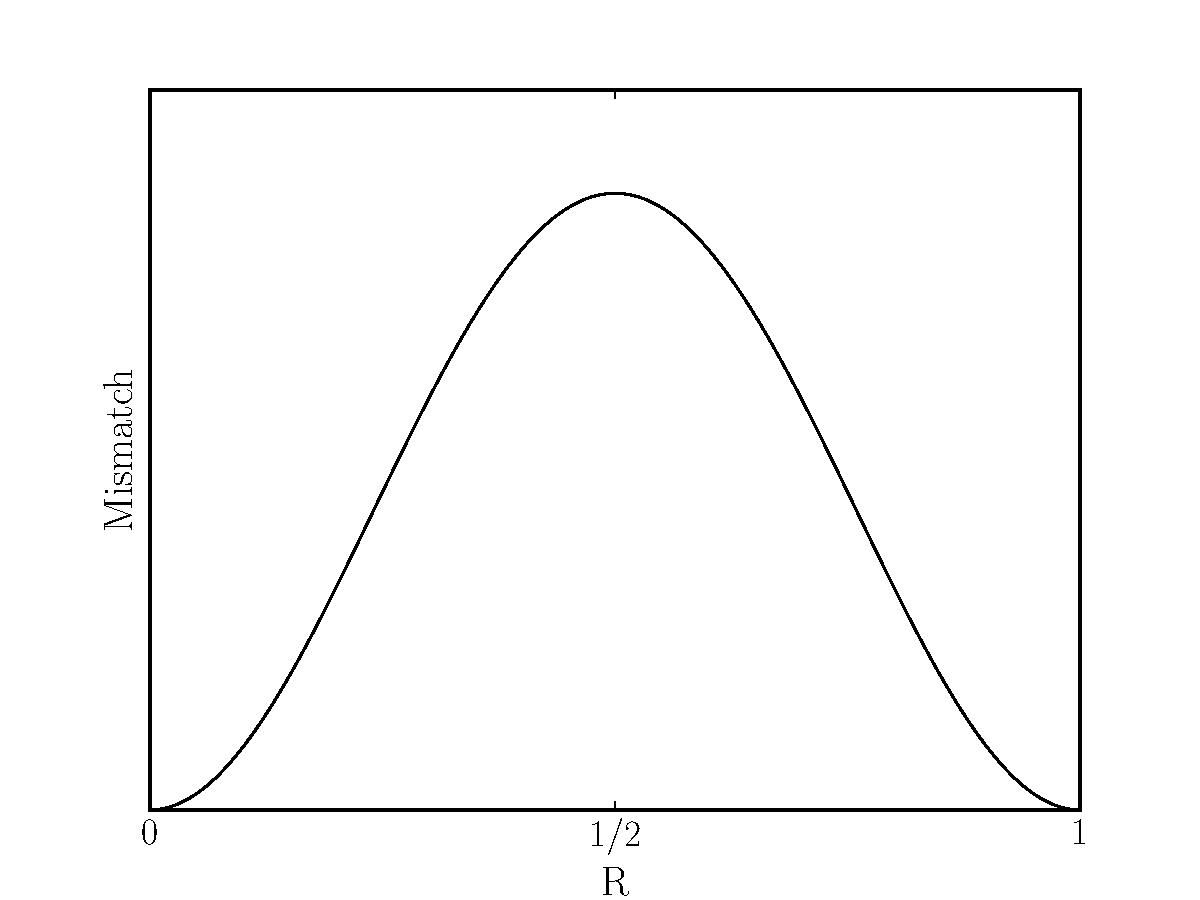
\includegraphics[width=.5\textwidth]{mismatch}
\caption{Illustration of the variation in mismatch over a single cycle with R}
\label{fig: Lyne mismatch}
\end{figure}

So far we have considered a simplistic, and highly unrealistic model. That is
measuring the mismatch over exactly one cycle. This is highly improbable in nature,
far more likely is to measure a fraction of a cycle. In Fig.~\ref{fig: Lyne mismatch kappa}
such a system is illustrated having defined $\kappa$ as the fraction of a cycle that
is observed. The calculation is not reproduced as it simply requires setting 
$T_{\mathrm{obs}} = \kappa T$ when calculating the mismatch.

\begin{figure}[ht]
\centering
\includegraphics[width=.5\textwidth]{mismatch_during_one_subdomain}
\caption{Illustration of the variation in mismatch with observation time 
parameterised by $\kappa$ the fraction of a cycle that we observe over.}
\label{fig: Lyne mismatch kappa}
\end{figure}
\FloatBarrier

\subsection{Extending the model to an arbitrary number of cycles} The phase
Having calculated the mismatch during a single cycle we now extend the calculation
to an arbitary number of cycles as described by equation \eqref{eqn: arbitrary full phase residual}

The parameter
space offsets will cycle $\bdl^{\alpha i} = \left[\bdl^{A i}, \bdl^{B i}, \bdl^{A i}, \dots \bdl^{Bi}\right]$.
The metric can be decomposed into four matrices $g_{AAij}$, $g_{ABij}$, $g_{BAij}$, and $g_{BBij}$, this
allows us to expand the mismatch calculation as follows
\begin{align}
m & = g_{\alpha \beta i j} \bdl^{\alpha i} \bdl^{\beta j} \\
& = \s{i=1}{2N}\s{j=1}{2N} g_{\alpha \beta i j} \bdl^{\alpha i} \bdl^{\beta j} \\
& = N\left(\s{j=1}{2N} g_{\alpha \beta A j} \bdl^{\alpha A} \bdl^{\beta j} + \s{j=1}{2N} g_{\alpha \beta B j} \bdl^{\alpha B} \bdl^{\beta j} \right) \\
& = N^{2}\left(g_{\alpha\beta AA} \bdl^{\alpha A} \bdl^{\beta A} + g_{\alpha \beta AB} \bdl^{\alpha A} \bdl^{\beta B} + g_{\alpha \beta BB} \bdl^{\alpha B} \bdl^{\beta B} + g_{\alpha\beta BA} \bdl^{\alpha B} \bdl^{\beta A}  \right)
\end{align}
Calculating the metric elements from equation~\eqref{eqn: metric} and inserting the parameter space offsets
\eqref{eqn: Lyne parameter space offsets} yields a mismatch given by
\begin{equation}
m(T, R, N) = \frac{\pi^{2}}{180}T^{4}\dST^{2} R^{2}\left(1-R\right)^{2} \left(N \left(18 R^{2} - 18 R + 6\right) - 5 \left(2 R - 1\right)^{2}\right)
\end{equation}
This expression is valid only for searches over an integer number of cycles which is nonphysical.
The behaviour of $m$ in-between cycles will oscillate about the linear growth in $N$ that 
can be interpolated from this expression. For our purposes it is enough to see that the mismatch 
grows approximately linearly over several cycles. 
